%========================%
%        Preamble        %
%========================%
\documentclass[12pt]{amsart}

    %========================%
%        Packages        %
%========================%

\usepackage[utf8]{inputenc}
%\usepackage{amsmath}    % Included in amsart package
%\usepackage{amsthm}     % 
\usepackage{amssymb}      % 
\usepackage{mathtools}      % Paired Limiter Macros
% \usepackage{mdframed}       % boxes for theorem
\usepackage{enumitem}     % Continuous numbering of lists
\usepackage[hidelinks]{hyperref}
\usepackage{tikz}
\usetikzlibrary{positioning}
\usepackage{blindtext}
\usepackage{graphicx}
\usepackage{float}

%========================% 
%          Title         %
%========================% 
\title{Chapters 31 and 32 Notes}
\author{Anish Sundaram}
\date{\today}

%========================% 
%        Theorems        %
%========================% 
\theoremstyle{definition}
\newtheorem{theorem}{Theorem}  % Boxed theorems
\newtheorem{definition}{Definition} % Definitions
\newtheorem{example}{Example}       %
\newtheorem{algorithm}{Algorithm}
\newtheorem*{proof*}{Proof}         % non-numbered
\newtheorem*{remark}{Remark}        %
\numberwithin{equation}{theorem}    % Local equation numbering

\setcounter{tocdepth}{3}      % Show subsubsections in contents

%========================% 
%        Macros          %
%========================% 
\DeclarePairedDelimiter\abs{\lvert}{\rvert}  % Vertical bars
\DeclarePairedDelimiter\norm{\lVert}{\rVert} % Double vertical bars
\newcommand{\drawvec}[1]{                    % matrices on one line
    \begin{bmatrix}
        #1
    \end{bmatrix}
}


% \begin{figure}[H]
%     \centering
%     \includegraphics[width=5in]{global-carbon-cycle.png}
%     \caption{The Global Carbon Cycle}
%     \label{global-carbon-cycle}
% \end{figure}

%========================% 
%         Document       %
%========================% 
\begin{document}
\maketitle

\tableofcontents

\section*{31 Alternating Current}
In this chapter we will learn how resistors, inductors, and capacitors behave in circuits with sinusoidally varying voltages and currents. Many of the principles that we found useful in Chapter 30 are applicable, along with several new con- cepts related to the circuit behavior of inductors and capacitors. A key concept in this discussion is \textit{resonance}, which we studied in Chapter 14 for mechanical systems.


\subsection*{31.1 Phasors and Alternating Currents}

\begin{definition}
    \textbf{Alternating Current}:
    an electric current that reverses its direction many times a second at 
    regular intervals, typically used in power supplies. Alternating current has a peak voltage and current,
    as well as an average. Alternating current is provided by an \textbf{AC Source}
\end{definition}

\begin{definition}
    \textbf{Voltage Amplitude}:
    Because Voltage alternated due to fluctuation in AC current it has a sinusoidally
    shape, being described by the equation $$u = Vcos(\omega t)$$ where $u$ is the instantaneous
    potential difference and $V$ is the maximum or peak voltage, sometimes designated as $V_0$
    \begin{remark}
        In the US and Canada the common frequency for distribution systems is $f$ = 60Hz orr 377 rad/s, while
        the rest of the world uses $f$ = 50 Hz ($\omega$ = 314 rad/s)
    \end{remark}
\end{definition}

\begin{definition}
    \textbf{Angular Frequency($\omega$)}:
    Angular Frequency is a scalar measure of rotation rate. It refers to the rate of change of the argument of the sine function
    Angular Frequency can be found by the equation $$\omega = 2\pi f$$ where $f$ is the frequency measured in Hz.
\end{definition}

\begin{definition}
    \textbf{Current Amplitude}:
    Much like Voltage the Current outputted by an AC battery varies with time and fluctuates in a sinusoidal fashion which can be described by the equation $$i = Icos(\omega t)$$ where $i$ is instantaneous currnet and $I$ is peak current, sometimes designated as $I_0$
\end{definition}

\subsubsection*{31.1.1 Phasor Diagrams}

\begin{definition}
    \textbf{Phasors and Phasor Diagrams}:
    To represent sinusoidally varying voltages and currents, we use rotating vector diagrams wherein the instantaneous value is represented by the projection onto a horizontal axis of a vector with a length equal to the amplitude of the quantity which rotates CCW with angular speed $\omega$. These rotating vectors are called \textbf{Phasors}.
\end{definition}

\begin{figure}[H]
    \centering
    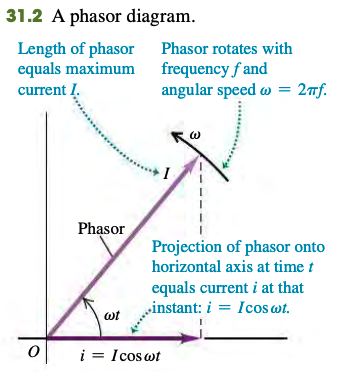
\includegraphics[width=3in]{Media/Phasor.png}
    \caption{Phase Diagram}
    \label{Phase Diagram}
\end{figure}

\subsubsection*{31.1.2 Recitified Alternating Current}

\begin{definition}
    \textbf{Rectified Average Current($I_{rav}$)}:
    Because it is dificult to measure alternating current in a Galvanometer we can use Recitified Average Current instead to measure. It can be computed by averaging the absolute value of a waveform over one full period of the waveform. or put into an equation as $$I_{rav} = \frac{2}{\pi}I = .637I$$ where $I$ is the current amplitude.
\end{definition}

\subsubsection*{31.1.3 Root-Mean-Square(rms) Values}

\begin{definition}
    \textbf{RMS Current and Voltage}:
    Another more useful way to describe the current and voltage(which can be both positive or negative) is the root-mean-square value, of which is never 0 unless i/u is zero at every instant. RMS Current can be defined as $$I_{rms} = \frac{I}{\sqrt{2}}$$ and RMS Voltage can be defined as$$V_{rms} = \frac{V}{\sqrt{2}}$$ In other words dividing the peak value by $\sqrt{2}$.
\end{definition}

\subsection*{31.2 Resistance and Reactance}

\begin{definition}
    \textbf{Inductive Reactance($X_L$)}:
    Inductive reactance is the name given to the opposition to a changing current flow by an inductor, it is measured in Ohms like resistance. Inductive Reactance is calculated by the equation 
    $$X_L = 2\pi f L = \omega L$$ where $L$ is the inductance. The amplitude of voltage across an inductor for AC Current can be found by $$V_L = IX_L$$
    \begin{remark}
        The peaks of Inductor voltage and current are out of phase by a quarter-cycle. Since the voltage peaks occur a quarter-cycle earlier than the current peaks, we say that the voltage leads the current by 90°
    \end{remark}
\end{definition}

\begin{definition}
    \textbf{Capacitive Reactance($X_L$)}:
    Capacitive reactance is the name given to the opposition to a changing current flow by an Capacitor, it is measured in Ohms like resistance. Capacitive Reactance is calculated by the equation 
    $$X_C = \frac{1}{2\pi f L} = \frac{1}{\omega C}$$ where $C$ is the Capacitance. The amplitude of voltage across an Capacitor for AC Current can be found by $$V_L = IX_C$$
    \begin{remark}
        The peaks of Capacitor voltage and current are out of phase by a quarter-cycle. Since the voltage peaks occur a quarter-cycle before than the current peaks, we say that the voltage trails the current by 90°
    \end{remark}
\end{definition}

\begin{remark}
    Greater reactance leads to smaller currents for the same voltage applied. 
\end{remark}

\begin{definition}
    \textbf{Phase Angle ($\phi$)}:
    The Phase Angle represents the fraction of the period that y lags or leads the function. In our case it is the phase of the voltage relative to current.
    \begin{enumerate}
        \item For a pure Resistor $\phi = 0$
        \item For a pure Inductor $\phi = 90$
        \item For a pure Capacitor $\phi = -90$
    \end{enumerate}
   
    \begin{remark}
        If the Circuit is more Capacitive then Inductive the Phase angle will be negative, opposite holds true as well.
    \end{remark}
\end{definition}

\subsection*{31.3 The L-R-C Series Circuit}

\begin{definition}
    \textbf{Impedance($Z$)}:
    The Impedance of an AC circuit is the effective resistance of an electric circuit or component to alternating current, arising from the combined effects of ohmic resistance and reactance. The general equation for Impedence is  $$Z = \sqrt{R^2 + (X_l - X_c)^2}$$ where $R$ is Resistance, $X_L$ is Inductive Reactance and $X_C$ is Capacitive Reactance. This can be used to find the total Current through an L-R-C or any derivative circuit through the equation $$V = IZ$$

    \begin{remark}
        To Find the Phase Angle of an L-R-C series Circuit the equation following can be used:
        $$tan\phi = \frac{X_L- X_c}{R}$$
    \end{remark}
\end{definition}

\begin{figure}[H]
    \centering
    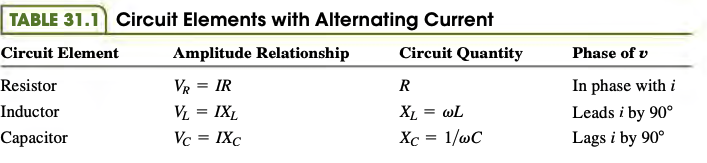
\includegraphics[width=5in]{Media/Elements.png}
    \caption{Phase rules of Circuit Elements}
    \label{Phase Rules of Circuit Elements}
\end{figure}

\subsection*{31.4 Power in AC Circuits}

\begin{remark}
    There is no power dissipated by a Capacitor or an Inductor as both absorb and release charge similar to a battery, and thus no power dissipates unlike a resistor.
\end{remark}

\begin{definition}
    \textbf{Average Power into a AC Circuit}:
    The average power into a general AC circuit can be calculated using the following equations:
    $$P_{aV} = .5VIcos\phi = V_{rms}I_{rms}cos\phi$$
\end{definition}

\begin{definition}
    \textbf{Power Factor}:
    The ratio of the actual electrical power dissipated by an AC circuit to the product of the r.m.s. values of current and voltage. The factor $cos\phi$ is called the power factor. 
\end{definition}

\subsection*{31.5 Resonance in AC Circuits}

\begin{definition}
    \textbf{Resonance}:
    The peaking of the current amplitude. The angular frequency $\omega_0$ at which the resonance peak occurs is called the \textbf{resonance angular frequency}. The Resonance Angular Frequency can be found by the equation $$\omega_0 = \frac{1}{\sqrt{LC}}$$
\end{definition}

\begin{definition}
    \textbf{Resonance Frequency ($f_0$)}:
     is when $X_L$ is equal to $X_C$. Resonance Frequency is found by the equation 
     $$f_0 = \frac{\omega_0}{2\pi} = \frac{1}{2\pi \sqrt{LC}}$$

     \begin{remark}
         When a circuit is at resonance frequency the inductive reactance and capacitive reactace are the same and thus negate eachother, so the only impedence comes from the resistor and the reactance is null.
     \end{remark}
\end{definition}

\subsection*{31.6 Tranformers}

    \begin{definition}
        \textbf{Transformers}:
        A transformer is used to transform the voltage and current levels in an ac circuit. In an ideal transformer with no energy losses, if the primary winding has N1 turns and the secondary winding has N2 turns, the amplitudes (or rms values) of the two voltages are related.
        The relations used by transformers are:
        $$\frac{V_2}{V_1} = \frac{N_2}{N_1}$$
        and
        $$V_1I_1 = V_2I_2$$
        and
        $$\frac{N_1}{N_2} = \frac{I_2}{I_1}$$
        For all of which 1 is the primary and 2 is the secondary.
        \begin{remark}
            The Efficiency of a Transformer can be found by the following:
            $$\frac{P_1}{P_2} * 100$$ where $P_1$ is initial power for the
            primary coil and $P_2$ is the power of the secondary coil.
        
        \end{remark}
    \end{definition}


\section*{32 Electromagnetic Waves}
Maxwell’s equations show that a time-varying magnetic field acts as a source of electric field and that a time-varying electric field acts as a source of magnetic field. These $\vec{E}$ and $\vec{B}$ fields can sustain each other, forming an \textit{electromagnetic wave} that propagates through space. Visible light is one example of an electromagnetic wave; other kinds are produced by wi-fi base stations, x-ray machines, and radioactive nuclei.

\subsection*{32.1 Maxwell's Equations and Electromagnetic Waves}

\begin{definition}
    \textbf{Electromagnetic Wave/ Electromagnetic Radiation}:
    When either an electric or a magnetic field is changing with time, a field of the other kind is induced in adjacent regions of space as shown by Ampere's Law. This disturbance of time-varying electric and magnetic fields that can propagate through space from one region to another have the properties of a wave, an EM wave.
    \begin{remark}
        An EM wave can travel even when there is no matter in the intervening region.
    \end{remark}
\end{definition}

\begin{definition}
    \textbf{Maxwell's Equations}:
    The Complete versions of previous equations
    \begin{enumerate}
        \item Gauss's Law for $\vec{E}$: $$\oint \vec{E} \cdot d\vec{A} = \frac{Q_{encl}}{\epsilon_0}$$ 
        \item Gauss's Law for $\vec{B}$: $$\oint \vec{B} \cdot d\vec{A} = 0$$
        \item Farada's Law for stationary integration path:$$\oint \vec{E} \cdot d\vec{l} = -\frac{d\Phi_B}{dt}$$  
        \item Ampere’s law for a stationary integration path:
        $$\oint \vec{B} \cdot d\vec{l} = \mu_0 (i_c + \epsilon_0\frac{d\Phi_E}{dt})encl$$ where $i_c$ is the conduction current through the path.
    \end{enumerate}
\end{definition}

\begin{definition}
    \textbf{EM Spectrum}:
    The length of EM waves of all frequencies and wavelengths, ranging from Radio and Tv waves on the high end of wavelength to Gamma rays on the low end.
    \begin{remark}
        Recall that the equation relating Wavelength, Frequency, and velocity is $$v = f\lambda$$ where in a vacuum all waves have the same propagation speed $$c = 299,792,458 m/s = 3*10^8 m/s$$ so we get $$c = \lambda f$$
    \end{remark}
\end{definition}

\begin{figure}[H]
    \centering
    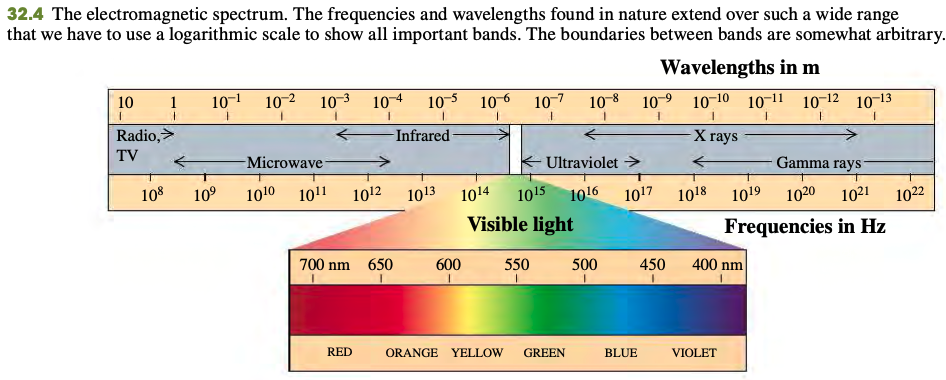
\includegraphics[width=5in]{Media/EMSpectrum.png}
    \caption{Diagram of EM Spectrum}
    \label{Diagram of EM Spectrum}
\end{figure}


\begin{remark}
    Energy of a Photon can be found by the eqaution $$E = hF$$ where $h$ is Plank's constant 
    $h = 6.626*10^-{34} js$
\end{remark}

\subsection*{32.2 Plane EM Waves and the Speed of Light}



\begin{definition}
    \textbf{Plane Wave}:
    A physical quantity whose fields are constant over any plane that is perpendicular to the direction of propagation. The relation between the speed of such a wave and the resulting $\vec{B}$ and $\vec{E}$ fields can be found by the equation 
    $$E = cB$$ where $c$ is the speed of light in vacuum mentioned above.
    However, this relation only holds if E and B are related in some manner, additional methods to calculated $\vec{B}$ and $c$ are as follows:
    $$B - \epsilon_0\mu_0cE$$ and $$c = \frac{1}{\sqrt{\epsilon_0\mu_0}}$$
    of which $\epsilon_0$ and $\mu_0$ are the electric and magnetic constants respectively.
    \begin{remark}
        To satisfy Maxwell's equations any wave discussed must be a \textbf{Transverse wave}, which is a wave whose oscillations are perpendicular to the direction of the wave's advance. This is in contrast to a \textbf{longitudinal wave} which travels in the direction of its oscillations.
    \end{remark}
\end{definition}

\begin{figure}[H]
    \centering
    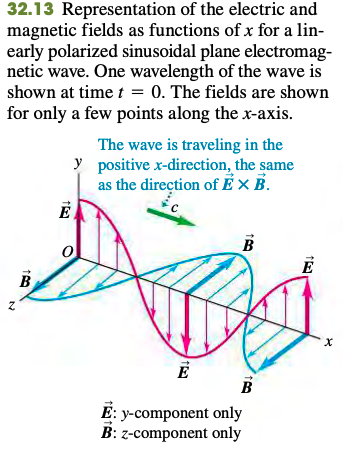
\includegraphics[width=3in]{Media/EM.png}
    \caption{Depiction of EM Wave}
    \label{Depiction of EM Wave}
\end{figure}

\begin{definition}
    \textbf{Key Properties of EM Waves:}
    \begin{enumerate}
        \item The wave is transverse; The direction of propagation is the direction of the vector product $\vec{E} \times \vec{B}$
        \item There is a definite ratio between the magnitudes of $\vec{E}$  and $\vec{B}$: $E = cB$.
        \item The wave travels in vacuum with a definite and uniform speed.
        \item Electromagnetic waves require no medium.
    \end{enumerate}
\end{definition}

\begin{figure}[H]
    \centering
    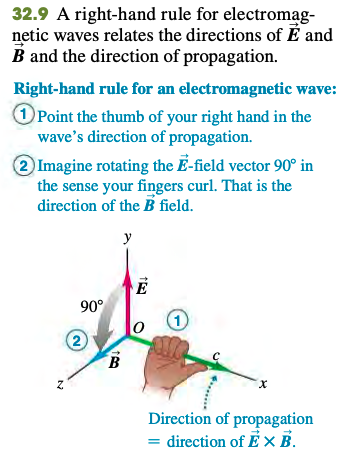
\includegraphics[width=3in]{Media/EMRHR.png}
    \caption{RHR for EM waves}
    \label{RHR for EM waves}
\end{figure}

\subsection*{32.3 Sinusoidal EM Waves}

\begin{definition}
    \textbf{Wave Functions in vacuum}:
    The functions to map the movement of the sinusoidal fields of EM plane waves propogating in the \textbf{+x} direction are as follows:
    $$\vec{E}(x,t) = \hat{j}E_{max}cos(kx-\omega t)$$
    and 
    $$\vec{B}(x,t) = \hat{k}B_{max}cos(kx-\omega t)$$
    where for both $k$ is the wave number and $\omega$ is the angular frequency.
    \begin{remark}
        Eaves propagating in the \textbf{-x} direction are as follows:
        $$\vec{E}(x,t) = \hat{j}E_{max}cos(kx+\omega t)$$
    and 
    $$\vec{B}(x,t) = -\hat{k}B_{max}cos(kx+\omega t)$$ 
    \end{remark}
\end{definition}

\subsubsection*{32.3.1 EM waves in Matter}

\begin{definition}
    \textbf{Speed of EM in Dialectric}:
    Although matter is not necessary for travel, it does impact speed. The new equation is as follows:
    $$v = \frac{1}{\sqrt{\epsilon\mu}} = \frac{1}{\sqrt{KK_m}}\frac{1}{\sqrt{\epsilon_0\mu_0}} = \frac{c}{\sqrt{KK_m}}$$
    wherein $\epsilon$ and $\mu$ are the permeability and permitivity and $K$ is the Dialectric constant and $K_m$ is relative permeability.$c$ is the speed of light in vacuum.
    \begin{remark}
        Because we are no longer in a vacuum $\mu_0$ must be replaced by $\mu = K_m\mu_0$ and thereby $E = vb$ and $B=\epsilon\mu vE$
    \end{remark}
\end{definition}

\begin{definition}
    \textbf{Index of Refraction}:
    The ratio of the speed $c$ in a material versus speed $v$ in vacuum:$$\frac{c}{v} = n = \sqrt{KK_m}$$
\end{definition}

\subsection*{32.4 Energy and Momentum in EM Waves}

\begin{definition}
    \textbf{Energy Density and Energy Absorbed}:
    The energy density of an Electric field can be found by the eqaution $$u_E = .5\epsilon_0E^2$$
    and the equation for the energy density of a Magnetic Field can be found by $$u_B = \frac{B^2}{2\mu_0}$$
    Thus the total energy density for a AM wave in vacuum is $$u =5\epsilon_0E^2 + \frac{B^2}{2\mu_0}$$ but because $u_E$ = $u_B$ the equation is simplified to $$u=\epsilon_0E^2$$
    \begin{remark}
        The total amount of energy absorbed by a surface can be found from the equation
        $$\Delta U = \epsilon_0cE^2At$$
    \end{remark}
\end{definition}

\subsubsection*{32.4.1 The Poynting Vector, Power, and Intensity}
\begin{definition}
    \textbf{Poynting Vector($\vec{S})$}:
    A vector quantity that describes both the magnitude and direction of the energy flow rate. Found by the equation
    $$\vec{S}=\frac{1}{\mu_0}\vec{E}\times\vec{B}$$ where the magnitude $$S = EB/\mu_0 =\frac{dU}{Adt} =\sqrt{\frac{\epsilon_0}{\mu_0}}E^2 = \epsilon_0CE^2$$ in a vacuum where the unit is $W/m^2$ 
    \begin{remark}
    The Average Poynting vector magnitude can be found by using:
    $$\bar{S} = .5S_0 = .5\epsilon_0CE_0^2 = .5\frac{c}{\mu_0}B_0^2=\frac{E_0B_0}{2\mu_0} = E_{rms}{B_rms}/\mu_0$$
    \end{remark}
\end{definition}

\begin{definition}
    \textbf{Power}:
    The total energy flow per unit time (power, P) out of any closed surface is the integral of S over the surface:
    $$P = \frac{\Delta U}{\Delta t} = \oint\vec{S}\cdot d\vec{A} $$
\end{definition}

\begin{definition}
    \textbf{Intensity}:
    Wave intensity is the average power that travels through a given area as the wave travels through space. The intensity of a sinusoidal EM wave in vacuum is 
    $$I = S_{av} = \frac{E_{max}B_{max}}{2\mu_0} = \frac{E_{max}^2}{2\mu_0c} = .5\sqrt{\frac{\epsilon_0}{\mu_0}}E_{max}^2 = 
    .5\epsilon_0cE_{max{^2}}$$ where $S_{av}$ is the magnitude of average Poynting vector. Units are $W/m^2$
\end{definition}

\subsubsection*{32.4.2 EM Momentum Flow and Radiation Pressure}

\begin{definition}
    \textbf{Flow rate of EM Momentum}:
    We’ve shown that electromagnetic waves transport energy. It can also be shown that electromagnetic waves carry momentum $p$. This Momemntum can be described by $$\frac{dp}{dV} = \frac{EB}{\mu_0c^2} = \frac{S}{c^2}$$ This momementum has a corresponding flow rate which can be described by 
    $$\frac{1}{A}\frac{dp}{dt} = \frac{S}{c} = \frac{EB}{\mu_0c}$$ where $\frac{1}{A}\frac{dp}{dt} $ is the Momentum transfered per unit surface area per unit time.
\end{definition}

\begin{definition}
    \textbf{Radiation Pressure}:
    Radiation pressure is the mechanical pressure exerted upon any surface due to the exchange of momentum between the object and the electromagnetic field. This includes the momentum of light or electromagnetic radiation of any wavelength that is absorbed, reflected, or otherwise emitted by matter on any scale. 
    $$\rho_{rad} = \frac{S_{av}}{c} = \frac{I}{c}$$ where $I$ is intensity for a wave totally absorbed and $$\rho_{rad} = \frac{2S_{av}}{c} = \frac{2I}{c}$$ for a wave totally reflected
\end{definition}

\subsection*{32.5 Standing EM Waves}

\begin{definition}
    \textbf{Standing Wave}:
    A Standing Wave is a wave which oscillates in time but whose peak amplitude profile does not move in space. The peak amplitude of the wave oscillations at any point in space is constant with time, and the oscillations at different points throughout the wave are in phase.
\end{definition}

\begin{definition}
    \textbf{Nodal Planes}:
    A node is a point along a standing wave where the wave has minimum amplitude.
    \begin{remark}
        \begin{enumerate}
            \item The Nodal Planes of $\vec{E}$ are $$x = 0, \frac{\lambda}{2}, \lambda, 
            \frac{3\lambda}{2},...$$
            \item The Nodal Planes of $\vec{B}$ are $$x = \frac{\lambda}{4}, \frac{3\lambda}{4},
            \frac{5\lambda}{4},...$$
        \end{enumerate}
        
    \end{remark}
\end{definition}




\end{document}
